%11_graphs.tex
%notes for the course PandA2 COMS10001 taught at the University of Bristol
%2016-7 Conor Houghton conor.houghton@bristol.ac.uk

%To the extent possible under law, the author has dedicated all copyright 
%and related and neighboring rights to these notes to the public domain 
%worldwide. These notes are distributed without any warranty. 

\documentclass[11pt,a4paper]{scrartcl}
\typearea{12}
\usepackage{graphicx}
\usepackage{listings}
\usepackage{tikz}
\usepackage{tkz-berge}
%\usepackage{tikz-qtree}                                                        
\usetikzlibrary{positioning}
\usetikzlibrary{arrows.meta}
\usetikzlibrary{shapes.geometric}
\lstset{language=C}
\pagestyle{headings}
\markright{COMS10001 - PandA2 11\_graphs - Conor}
\begin{document}

\subsection*{11- graphs\footnote{\texttt{http://github.com/conorhoughton/COMS10001}} - UNFINISHED}

Graphs are a useful way to represent data; there are powerful
algorithms for graphs and so by describing some type data as a graph
it becomes possible to process it using these algorithms. From a more
theoretical point-of-view, graphs present interesting problems to the
study of algorithms and some branches of mathematics, like
combinatorics; many graph theory problems have interesting and elegant
solutions while others are unsolved.

A graph is a set \textsl{nodes}, also called \textsl{vertices} linked
by \textsl{edges}. In an undirected graph, these edges have no
direction, as in Fig.~\ref{fig:graph}, in a directed graph, the edges
have direction, as in Fig.~\ref{fig:dir_graph} and in a weighted graph
the edges have a weight, as in Fig.~\ref{fig:wei_graph}. Facebook is
an undirected graph, since \lq{}friendship\rq{} is reciprocal, Twitter
is an directed graph since \lq{}following\rq{} is not reciprocal; the
distances between cities connected by train lines is weighted
graph. You can imagine other possibilities, like directed weighted
graphs and graphs where the nodes also have weights, but we will only
consider directed, undirected and weighted here.

A common way to describe a graph algebraically is to use the adjacency
matrix. This describes the connections between the nodes; for an undirected graph it is the matrix:
\begin{equation}
A_{ij}=\left\{\begin{array}{cl}1&i\mbox{ is connected to }j\cr0&\mbox{otherwise}
\end{array}\right.
\end{equation}
so there is a one in the matrix in the $i$th row and $j$th column if
the $i$th node is connected to the $j$th node. The graphs we have
drawn all have letters labeling the nodes, so obviously for the matrix
you need to number the nodes, here we'll just make $a$ node 1, $b$ node two and so on, with this adjacency matrix for the graph in Fig.~\ref{fig:graph} is
\begin{equation}
A=[A_{ij}]=\left(
\begin{array}{ccccc}
0&1&1&1&0\\
1&0&1&0&0\\
1&1&0&1&0\\
1&0&1&0&1\\
0&0&0&1&0
\end{array}
\right)
\end{equation}



\begin{figure}
\begin{center}
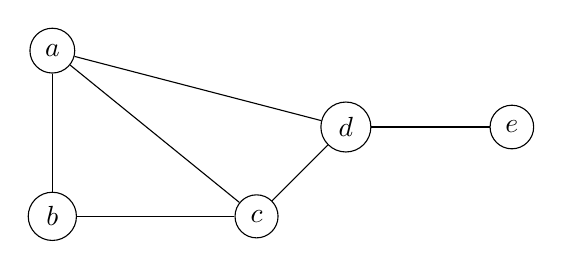
\begin{tikzpicture}
\node[draw,circle](a){$a$};
\node[draw,circle, below = 1.5cm of a](b){$b$};
\node[draw,circle, right =2cm of b](c){$c$};
\node[draw,circle, above right = 1cm of c](d){$d$};
\node[draw,circle, right = 1.5cm of d](e){$e$};
\path (a) edge (b);
\path (b) edge (c);
\path (c) edge (d);
\path (d) edge (e);
\path (a) edge (d);
\path (c) edge (a);
\end{tikzpicture}
\end{center}
\caption{A graph: this is an undirected graph so the edges have no
  direction. \label{fig:graph}}
\end{figure}

For a directed graph there is a one in the $i$th row and $j$ column of the adjacency matrix if there is a link from $i$ to $j$, so it is the matrix:
\begin{equation}
A_{ij}=\left\{\begin{array}{cl}1&i\mbox{ has an edge pointing to }j\cr0&\mbox{otherwise}
\end{array}\right.
\end{equation}
so, in the case of Fig.~\ref{fig:dir_graph} the matrix is 
\begin{equation}
A=\left(
\begin{array}{ccccc}
0&1&0&1&0\\
1&0&1&0&0\\
1&0&0&1&0\\
0&0&0&0&1\\
0&0&0&1&0
\end{array}
\right)
\end{equation}
In the weighted graph, as you might expect, the matrix entries correspond to the weights, so
\begin{equation}
A_{ij}=\left\{
\begin{array}{cl}
w&i\mbox{ is connected with weight }w\mbox{ to }j\cr 
0&\mbox{otherwise}
\end{array}\right.
\end{equation}
so the matrix is
\begin{equation}
A=\left(
\begin{array}{ccccc}
0&5&6&3&0\\
5&0&2&0&0\\
6&2&0&8&0\\
3&0&8&0&1\\
0&0&0&1&0
\end{array}
\right)
\end{equation}

\begin{figure}
\begin{center}
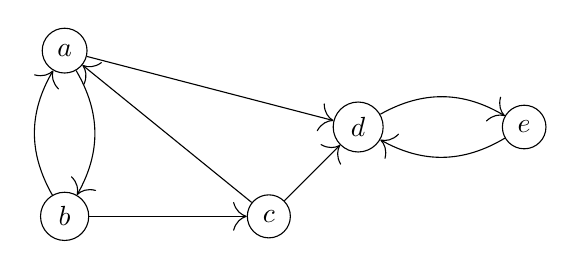
\begin{tikzpicture}
\node[draw,circle](a){$a$};
\node[draw,circle, below = 1.5cm of a](b){$b$};
\node[draw,circle, right =2cm of b](c){$c$};
\node[draw,circle, above right = 1cm of c](d){$d$};
\node[draw,circle, right = 1.5cm of d](e){$e$};
\path (a) edge[-{>[scale=2]},bend left] (b);
\path (b) edge[-{>[scale=2]},bend left] (a);
\path (b) edge[-{>[scale=2]}] (c);
\path (c) edge[-{>[scale=2]}] (d);
\path (d) edge[-{>[scale=2]},bend left] (e);
\path (e) edge[-{>[scale=2]},bend left] (d);
\path (a) edge[-{>[scale=2]}] (d);
\path (c) edge[-{>[scale=2]}] (a);
\end{tikzpicture}
\end{center}
\caption{A directed graph. \label{fig:dir_graph}}
\end{figure}

For an undirected graph the \textsl{degree} of a node is the number of
edges incident to it. Thus, for the graph in Fig.~\ref{fig:graph} the
node $a$ has degree three, $b$ has degree two, $c$ three, $d$ three
and $e$ has degree one. The degree is an important quantity for
describing graphs, though it won't be discussed here, often in
applications of graph theory dynamics on a graph is considered, for
example, epidemiological models are run on graphs were the nodes are
people and the edges contact, so, for a sexually transmitted disease
an edge would link two people who had had sex, in a disease that is
spread by aerosol it would link two people who had been in the same
room. For models like this the average degree of the nodes, and the
distribution of degrees, has a strong effect on the dynamics. The
degree can also be defined for directed graphs, for a directed graph
the degree is the number of incoming edges minus the number of
outgoing, so, for the graph in Fig.~\ref{fig:dir_graph} the degree of
$a$ is zero, whereas the degree of $b$ is -1.



Here we will be concerned with paths through graphs, it is possible to
give careful definitions of what we mean, but the ideas are intuitive
and clear enough to make do with less formal definitions. A
\textsl{walk} is a series of nodes and edges so that each node is
connected to one end of the subsequent edge and the node after that to
the other end, that is, it is a path going from node to node along
edges without any jumps. A \textsl{trail} is a walk in which no edge
is repeated. Here a \textsl{cycle} is a closed trail, that is a trail
that begins and ends at the same point; I say here because the term
cycle is sometimes used for a closed walk. Finally, a \textsl{tree} is
a graph with no cycles; trees are named because they are like trees, but not like the tree in Fig.~\ref{fig:not_a_tree}.

\begin{figure}
\begin{center}
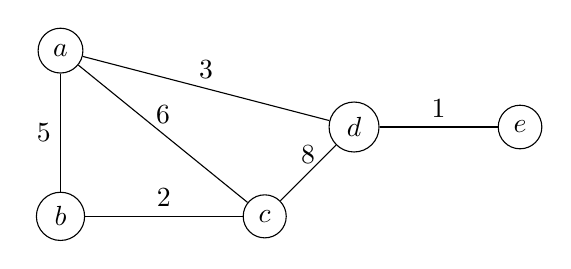
\begin{tikzpicture}
\node[draw,circle](a){$a$};
\node[draw,circle, below = 1.5cm of a](b){$b$};
\node[draw,circle, right =2cm of b](c){$c$};
\node[draw,circle, above right = 1cm of c](d){$d$};
\node[draw,circle, right = 1.5cm of d](e){$e$};
\path (a) edge node[left]{5} (b);
\path (b) edge node[above]{2} (c);
\path (c) edge  node[above]{8}(d);
\path (d) edge  node[above]{1}(e);
\path (a) edge  node[above]{3}(d);
\path (c) edge  node[above]{6}(a);
\end{tikzpicture}
\end{center}
\caption{A graph: this is a weighted graph so the edges have a value. \label{fig:wei_graph}}
\end{figure}

  

\begin{figure}
\begin{center}
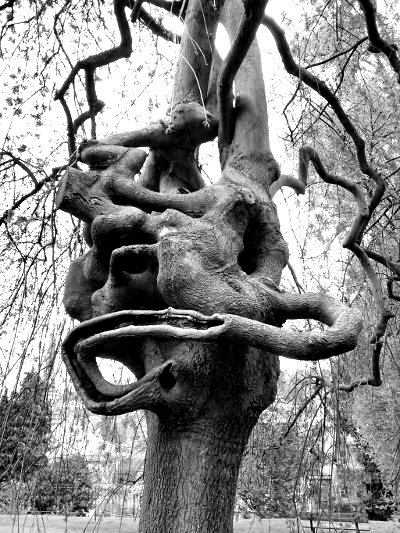
\includegraphics[width=6cm]{not_a_tree_bw.jpg}
\end{center}
\caption{This tree is not a tree, photographed in Hedgemead Park in Bath.\label{fig:not_a_tree}}
\end{figure}

\subsubsection*{Eulerian trees}

The subject of Eulerian trees is usually introduced through Euler's
original solution of the problem of the Seven Bridges of K\"onigsberg,
K\"{o}nigsberg, now Kalingrad, was a Prussian town where, as the story
is told, the townsfolk liked to walk in the evening over the seven
bridges in the town that connected a city which spanned two banks of
the river Pregel, along with two islands in the river. The layout is
shown in Fig.~\ref{fig:konigsberg}. The townsfolk sometimes wondered
if there was a route that would allow them to cross all the bridges,
but each bridge only once. The great mathematician Euler solved this
problem in 1736 by reducing it to a problem in graph theory, he
observed that what mattered was the bridges, not the land, so he
reduced the four land areas to nodes and thought of the bridges as
island. This graph is shown in Fig.~\ref{fig:konigsberg_graph}.

  

\begin{figure}
\begin{center}
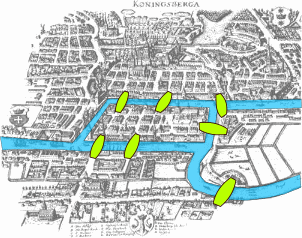
\includegraphics[width=6cm]{Konigsberg_bridges.png}
\end{center}
\caption{A picture of historical K\"{o}nigsberg with its seven bridges [from wikipedia].\label{fig:konigsberg}}
\end{figure}



\begin{figure}
\begin{center}
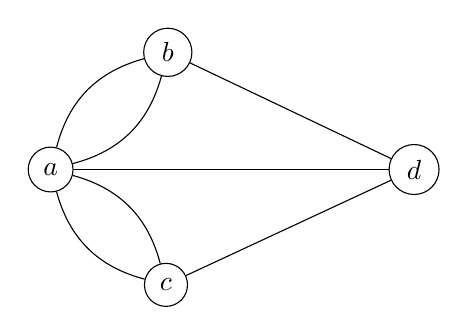
\begin{tikzpicture}
\node[draw,circle](a){$a$};
\node[draw,circle, above right = 1.5cm of a](b){$b$};
\node[draw,circle, below right = 1.5 cm of a](c){$c$};
\node[draw,circle, right = 4cm of a](d){$d$};
\path (a) edge[-,bend right] (b);
\path (a) edge[-,bend left] (b);
\path (a) edge[-,bend right] (c);
\path (a) edge[-,bend left] (c);
\path (a) edge[-] (d);
\path (d) edge[-] (b);
\path (d) edge[-] (c);
\end{tikzpicture}
\end{center}
\caption{The Bridges of K\"{o}nigsberg graph. \label{fig:konigsberg_graph}}
\end{figure}

Now, Euler reasoned like this: the townsfolk might start at one node
and end at another, but for the other two nodes they needed to leave
as often as they arrived, thus each visit used up two edges, one to
arrive by and one to leave. In other words, if you imagine removing
edges when the corresponding bridge has been traversed, visiting a
node reduced its degree by two, when all the bridges had been crossed
the degree of all the nodes must be reduced to zero, so unless a node
represents the starting point or end point, it must have an even
degree. Thus, if more than two nodes have odd degree, there is no
trail that includes every edge. In the case of K\"{o}nigsberg all the
nodes are odd, so there is no way the townsfolk can design a path that
crosses every bridge exactly once.

These days an \textsl{Eulerian trail} is a trail that visits every
node and an \textsl{Eulerian cycle} is a cycle that does the same. The
discussion of K\"{o}nigsberg above can be reformulated as a Theorem
which states that a graph cannot have an Eulerian trail unless all the
nodes have even degree or exactly two nodes have odd degree; a graph
cannot have an Eulerian cycle unless all the nodes are even. In fact
this theorem words the other way too, if a graph has only even degrees
there is an Eulerian cycle, if it has two odd degree nodes it has an
Eulerian trail starting at one odd node and ending at the other. We
won't prove this, or formalize the proof above, but we will consider a
construction for the Eulerian trail if there is one. Incidentally Thilo Gross from Eng Math found and walked an Eulerian trail for Bristol, he recounts his walk here: \texttt{http://www.reallygross.de/node/81}.

The Eulerian trail uses every edge, this suggests a similar problem,
the construction of a trail that visits every node exactly once. This
type of trail is called a Hamiltonian trail and the problem of whether
a graph has one is hard. Hamilton himself found a Hamiltonian trail
for a graph that has the same connectivity as the surface of dodecahedron: this puzzle is given in Fig.~\ref{fig:hamiltonian}.

\begin{figure}
\begin{center}
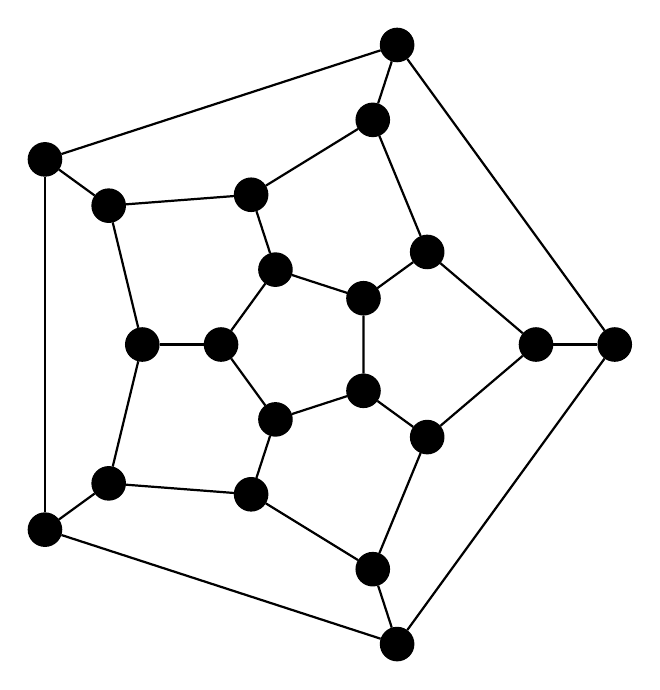
\begin{tikzpicture}
\GraphInit[vstyle=Simple]
        \grDodecahedral[form=2] 
\end{tikzpicture}                  
\end{center}
\caption{The Hamiltonian Game, a C19 puzzle which challenges you to find a trail that visits each node exactly once.\label{fig:hamiltonian}}
\end{figure}
\end{document}
